\documentclass{article}
\usepackage{biblatex}
\usepackage{graphicx}
\addbibresource{prosem.bib}
\begin{document}
\section{Non-Linear Filters}
Non-linear filters serve as additional ways of filtering images. Linear filters can work exceptionally well for certain cases, however one will encounter scenarios where using Non-Linear filters will lead to a better result both visually (Image Processing) and performance-wise. One example noise removal, but more on that later. First of all it is important to look at what non-linear filters actually are.

\subsection{What are Non-Linear Filters?}
First and foremost, what are Non-Linear filters? As mentioned previously, linear filters are filters where the signal-response of two signals and the sum of the responses to the two signals individually are the same. Based on that one may probably guess that non-linear filters are filters where this criteria is not satisfied, and this is the case. This could mean that, in relation to the input data, the transformation could, for instance, be exponential as opposed to linear. This can lead to bigger difficulties concerning frequency response analysis,\cite[p.~132]{szeliski} shift-invariance, etc.
\subsection{Some different types of Non-Linear filters}
\subsubsection{Median Filtering}
Consider a scenario with so-called salt and pepper noise, i.e. an image with noise consisting of sporadic black and white pixels. Were one to use for instance a Gaussian filter, one would quickly end up with a slightly blurred version of the original image (See fig 3.1). The noise would most likely still be there, simply in a slightly blurred format. Somewhat of a disappointment. There are however other methods of filtering, and for this scenario, a median filter would most likely do the trick.

\begin{figure}[!hb]
    \centering
    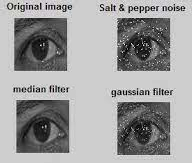
\includegraphics[width=0.5\linewidth]{medianfiltering.jpeg}
    \caption{Figure 3.1}
    \label{fig:enter-label} 
\end{figure}
Now we have seen an example median filtering, compared to Gaussian filtering, for a specific scenario, and what it does, it is time to dive into what a \textit{median filter actually is}. The algorithm works in this way: Given an input signal, in this case an image, it goes through every single pixel of the image, and replaces the value with the median value of the adjacent pixels (See fig 3.2). One can also let it go through the image whilst checking adjacent pixels in a 3px, 10px, or generally X-pixel radius around the current one, and replace it with the median of the pixels inside this X-pixel radius. The "X-pixel radius" is called a kernel. Increasing the kernel-size of the filter might lead to a "smeared" and somewhat blurry look in many scenarios, as in Figure 3.3
\begin{figure}
    \centering
    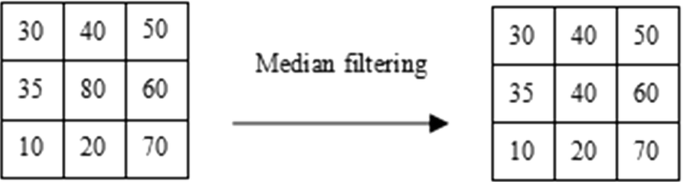
\includegraphics[width=0.5\linewidth]{medianfiltering.PNG}
    \caption{Figure 3.2 - Illustration of how the mean filter algorithm works}
    \label{fig:enter-label}
\end{figure}
\begin{figure}
    \centering
    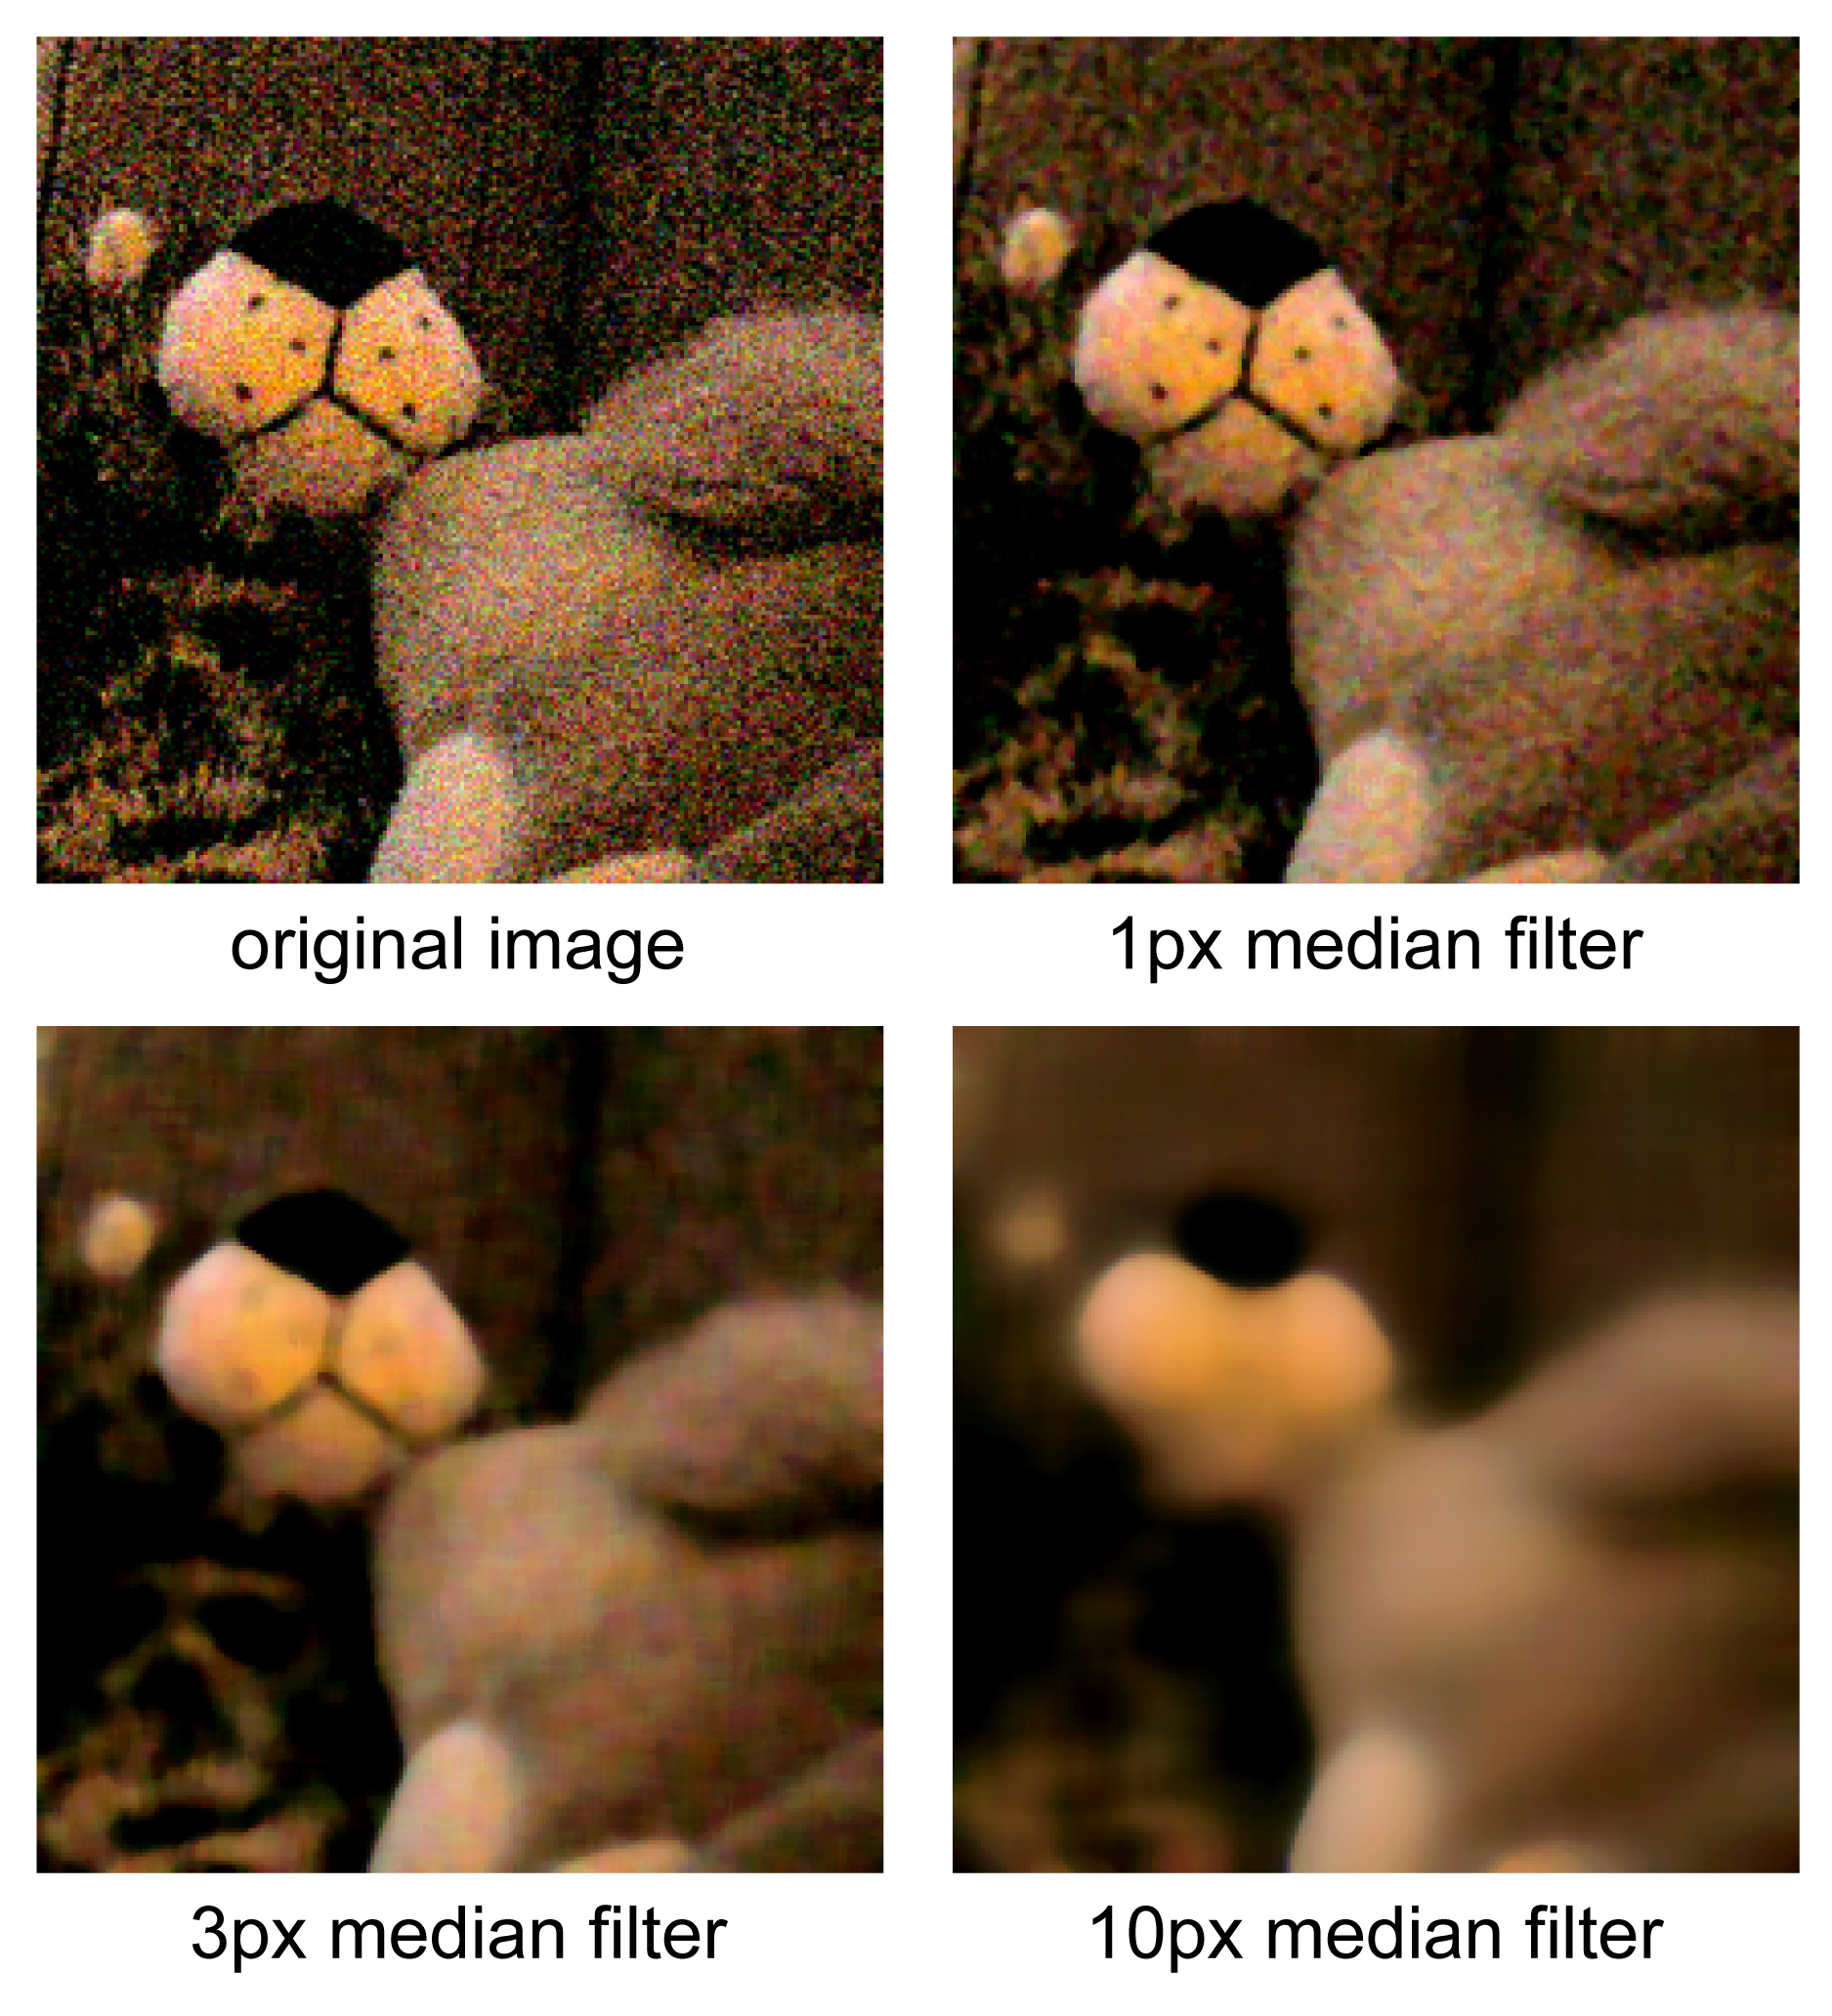
\includegraphics[width=0.5\linewidth]{median_example.jpg}
    \caption{Figure 3.3}
    \label{fig:enter-label}
\end{figure}
However, even though median filters work relatively well for this specific scenario, the cure for cancer is yet to be found. There are (several) scenarios in which median filters might produce sub-optimal results.

\subsubsection{Bilateral Filtering}
Another type of Non-Linear filter is the bilateral filter. In order to properly understand the bilateral filter, it is first important to understand a few other principles.

It would, at this point, be prudent to mention a certain property of filters that can be very much sought after, namely, \textit{edge-preservation}. When filtering away noise one often runs the risk of losing the clarity of the edges in the image. Given an image with a coin (Figure 3.4), and some noise, one might filter away the noise with a filter, perhaps a Gaussian would work here. After applying the filter, the noise might have been cleared away, but one will often recognize a certain "smudgyness" by the edges. The, perhaps, once sharp clear edges where the coins meet the background have seemingly melted more into their surroundings. Somewhat problematic. Applying an even stronger filter might remove the clear edge of the coins completely, making the coins look more like the sun in the middle of day than the coins they supposedly are.
\begin{figure}
    \centering
    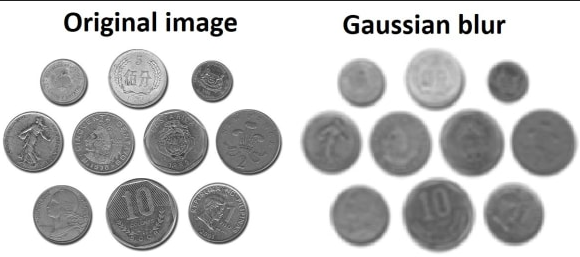
\includegraphics[width=0.5\linewidth]{coins.PNG}
    \caption{Figure 3.4 - Applying a Gaussian-filter has made the edges of the coins (against the background) less pronounced}
    \label{fig:enter-label}
\end{figure}

Another important filtering method to recognize, at this point, is weighted kernel filtering. Weighted kernel filtering is an extension of the median filter. It works by \textit{weighting} pixels based on their distance from the middle. I.e. the further the pixel is from the center, the smaller the effect of it, but importantly, it still has an influence!

Now to bilateral filters themselves. The base principle of bilateral filtering is applying the concept of weighted median filtering, yet with a tweak. The bilateral filter rejects values that are too much of an outlier for the current kernel, hence, often preserving edges better than the previously mentioned filters. Since a median filter uses all pixel-values in the kernel when processing an image, it may very well lead to blurred edges. Imagine, for instance, the aforementioned example with the coins (Figure 3.4). When the median filter does it's magic on the edges, for instance where the coin meets the background, it will use the values of the white background, and mix it into the values of the darker coins edges. Ergo, the edge of the darker coin will turn into a lighter colour because of the influence of the background. Apply the median filter several more times, and this will happen again and again and again, quickly leading to an unrecognizable blur, rather than a crisp clear image of coins with the noise removed (Note: This will most likely happen regardless of filter if one applies it an excessive amount of times, but the amount of times one must apply the filter for the image to become unrecognizably blurry or smudge-like is different).

Let's consider filtering the same image with a bilateral filter. When the bilateral filter considers pixels along the edge of the coins in Figure 3.4 it will not consider outliers, hence, it will not consider the pixels of the strong white background, rather focusing on the pixels of the coin itself, as they are more similar to the relevant pixel. That is not to say that applying the bilateral filter an exorbitant amount of times won't lead to the edges eventually blending into their surroundings, but the bilateral filter does, for most intents and purposes, preserve edges.


\subsubsection{Minimum- and Maximum Filtering}
Two more types of non-linear filters are minimum- and maximum filters. These two filters are often also called dilation and erosion filters, respectively. They are classified amongst the so called morphological filters. In many ways, the minimum and maximum filters are two sides of the same coin, they are very similar in all but one point. As the minimum filter moves along the image, processing as it should, it simply chooses the smallest value inside the current kernel and applies this value to the relevant pixel. Maximum filters work very similarly, but, as one might guess, they instead pick the largest value and assigns that to the relevant pixel. Given the two filters other names, dilation and erosion, it might not be too much of a leap to assume what an image processed by these filters would look like relative to the original. Minimum filters, or dilation filters, simply dilate the darker areas of images (since darker values tend to be assigned lower numbers). Effective if one wishes to thicken the borders of a dark-coloured letter on a light background in an image. Contrarily, the maximum filter, or erosion filter, will erode darker pixels from images. If a black pixel is surrounded by only white pixels, it will be gone after an erosion filter has been applied.
Lastly on minimum and maximum filters, a bit about binary images. What are binary images? They are in fact part of what led to the creation of morphological filters such as the here discussed minimum and maximum ones. As one might deduce from the name "binary images"  they operate with \textit{only} binary values. In other terms, each pixel can only have one of two values, black and white. Figure 3.6 demonstrates the application of the dilation and erosion filters on a binary image.
\begin{figure}[!hb]
    \centering
    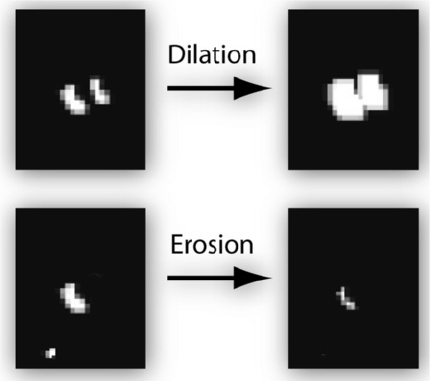
\includegraphics[width=0.5\linewidth]{minmax1.png}
    \caption{Figure 3.5 illustrates the usage of minimum and maximum filters}
    \label{fig:enter-label}
\end{figure}

\begin{figure}[!hb]
    \centering
    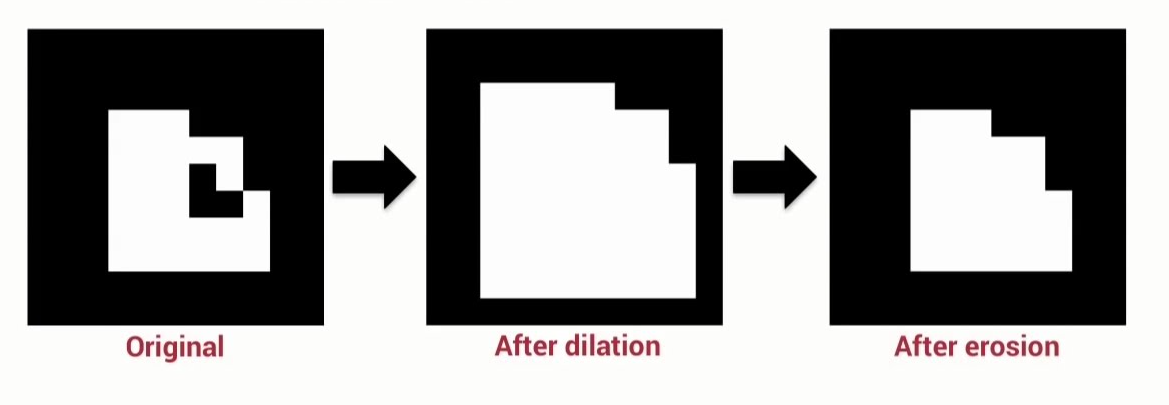
\includegraphics[width=0.5\linewidth]{minmax2.PNG}
    \caption{Figure 3.6 using a minimum filter succeeded by a maximum filter fills the gaps in the figure and then decreases it's size}
    \label{fig:enter-label}
\end{figure}
\subsubsection{Mean Shift Filtering}
Placeholder text

\subsubsection{Cellular Automata}
Cellular automata is something one probably has heard about in other contexts than image processing. Tracing it roots back to the late 40s, as the brainchild of the two late great scientists Stanislaw Ulam, and of course, the father of computer science himself Neumann Janos, commonly known as John von Neumann. Von Neumann was working on self-replicating-systems when he, with some help from Ulam, came up with his Cellular Automaton. Proving that his self-replicating automaton would work. But how can one apply this seemingly unrelated part of computer science to image processing?  First of all, let's assess how cellular automata work.

In essence, cellular automata are grids of cells, each containing what can be considered a finite state machine. They can be very useful in the analysis of many different systems, as well as in the fields of physics and biology. 
Now how specifically does one apply a cellular automaton to image processing?  As of now one of the most major application areas is noise removal in binary images.


\subsection{Optimal Non-Linear filtering}
Placeholder text

\subsection{Typical applications of Non-Linear filters}
The subject of where one can apply Non-Linear filters has already been touched upon. Likely, the most prominent application area of non-linear filters is in noise filtering.
\end{document}